\section{CLI backend for Rainbow interpreter}

%\subsection{Promotion on CLI}
%
%Implementing promotion on top of CLI is not straightforward, as it needs to
%patch and modify the already generated code, and this is not possible on .NET.
%
%To solve, we do xxx and yyy etc. etc.
%

\subsection{Flexswitches}

As already explained, \dacom{I guess flexswitches will be introduced
  in the previous sect.} \emph{flexswitch} is one of the key
concepts allowing the JIT compiler generator to produce code which can
be incrementally specialized and compiled at run time.

A flexswitch is a special kind of switch which can be dynamically
extended with new cases; intuitively, its behavior can be described
well in terms of flow graphs. Indeed, a flexswitch can be considered 
as a special flow graph block where links to newly created blocks are
dynamically added whenever new cases are needed. \dacom{in theory links could also be removed, but I
  do not know whether this possibility has been considered in Rainbow}

\begin{figure}[h]
\begin{center}
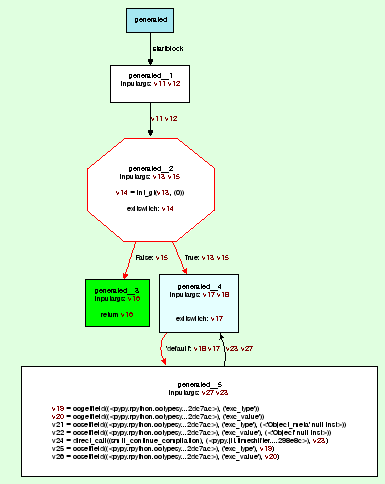
\includegraphics[height=5cm]{flexswitch1}
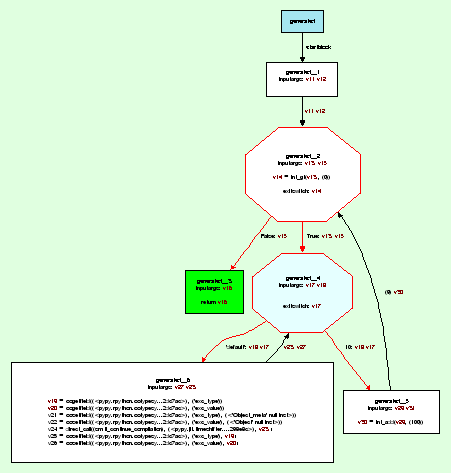
\includegraphics[height=5cm]{flexswitch2}
\caption{An example of a flexswitch evolution: in the picture on the
  right a new block has been dynamically added.}\label{flexswitch-fig}
\end{center}
\end{figure}

In the pictures of Figure~\ref{flexswitch-fig}, the cyan block
corresponds to a flexswitch; initially (picture on the left) 
only the block containing the code to restart the JIT compilation
is connected to the flexswitch; the picture on the right
shows the graph after the first case has been dynamically added to the flexswitch,
by linking the cyan block with a freshly created new block.


\subsection{Implementing flexswitches in CLI}

Implementing flexswitches for backends generating assembly code is
quite straightforward: basically, a new jump has to be inserted in the
existing code to point to the newly generated code fragment.

Unfortunately, the CLI VM does not allow modification of code which
has been already loaded and linked, therefore the simplest approach
taken for low level architectures does not work for higher level 
virtual machines as those for .NET and Java.

Since in .NET methods are the basic units of compilation, a possible
solution consists in creating a new method 
any time a new case has to be added to a flexswitch.
\dacom{comment for Antonio: I am not sure this is the best solution. This cannot work for Java where classes are the basic
  units}

\dacom{I still have to polish what comes next}

\newcommand{\commentout}[1]{}
\commentout{
Because of all these constraints we cannot simply map each graph to its own method, since we saw that our graphs can grow after they have already been executed few times.

Hence, we need to distinguish between the two concepts:

        * a graph is the logical unit of code as seen by the JIT compiler: concretely, the CLI JIT backend renders it as one or more methods;
        * a method is a collection of basic blocks; each method has the so called parent graph, i.e. the graph its blocks logically belongs to.

The first method of a graph is called main method (which has nothing to do with the Main static methods found in .exe files); other methods are called children methods.

When we want to add a new case to the flexswitch, we create a method containing all the new code; then we wrap the method inside a delegate (the .NET equivalent of a function pointer) and pass it to the flexswitch, so that it can later invoke it.
The hard bit: non-local links

Using this approach, after a while the blocks of our original graph are scattered over a lot of different methods; however, there are no constraints about how these blocks can be linked together, so it happens to have links between blocks which are not in the same method. In the following, we will refer to them as non-local links.

If the non-local block we want to jump to happens to be at the beginning of its containing method, it is enough to invoke the method; but, what if we want to jump somewhere in the middle? What we really want is to produce a method which has multiple entry-points; again, doing it in assembly would be trivial, but the virtual machine does not provide any support for it, so we need a work around.

Each method in a graph is assigned an unique 16 bit method id; each block in a method is assigned a progressive 16 bit block number. From this two numbers, we can compute the block id as an unsigned integer, by storing the method id in the first 16 bits and the block number in the second 16 bits. By construction, the block id is guaranteed to be unique in the graph.

The following picture shows a graph composed of three methods; the id of each method is shown in red, while the block ids are shown in red (for the method id part) and black (for the block number part). The graph contains three non-local links; in particular, note the link between blocks 0x00020001 and 0x00010001 which connects two block that resides in different methods.

Every method contains a special dispatch block, (not shown in the picture above) whose goal is to jump to the specified block number inside the method itself. The first argument of a child method is always a block id; when the method starts, it immediately jumps to the dispatch block, and thus to the desired block.

For example, suppose to have a method which contains 3 blocks numbered 0, 1, 2; here is how its dispatch blocks looks like; for simplicity it is shown as C# code, but it is actually generated as IL bytecode:

// dispatch block
int methodid = (blockid & 0xFFFF0000) >> 16); // take the first 16 bits
int blocknum = blockid && 0x0000FFFF;         // take the second 16 bits

if (methodid != MY_METHOD_ID) {
// jump_to_unknown block
...
}

switch(blocknum) {
case 0:
goto block0;
case 1:
goto block1;
case 2:
goto block2;
default:
throw new Exception("Invalid block id");
}

Whenever we want to jump to a non-local block, it is enough to store the block id in the appropriate variable and jump to the dispatch block. If the block resides in a different method, the jump_to_unknown block is entered; this special block is implemented differently by the main method and the child methods, as we will see soon.

Each time a new method is added to the graph, we build a delegate for it, and store it in a special array called method_map; since we assign the method id sequentially starting from 0, we are sure that to fetch the method whose id is n we can simply load the n-th element of the array.

The jump_to_unknown block of the main method uses this array to select the right method, and calls it (FlexSwitchCase is the type of delegates for all children methods):

// jump_to_unknown block of the main method
FlexSwitchCase meth = method_map[methodid];
blockid = meth(blockid, ...); // execute the method
goto dispatch_block;

Each child method returns a block id specifying the next block to jump to; after its execution, we assign the return value to the blockid variable, and jump again to the dispatch block, which will jump again to the appropriate block.

Keeping this in mind, it is straightforward to implement the jump_to_unknown block of children methods: it is enough to return the target block id to the caller, and let its dispatch loop do the right thing. If the caller is also a child method, it will return it again, until we reach the dispatch loop of the main method, which will finally do the jump. In theory, we could implement things differently and jumping directly from a child method to another one, but in that case the call stack could grows indefinitely in case of a tight loop between two blocks residing in different methods.

To implement the dispatch block we can exploit the switch opcode of the CLI; if the .NET JIT is smart enough, it can render it using an indirect jump; overall, jumping to a non-local block consists of an indirect function call (by invoking the delegate) plus an indirect jump (by executing the switch opcode); even if this is more costly than a simple direct jump, we will see in the next section that this not the main source of overhead when following a non-local link.

Obviously, the slow dispatching logic is needed only when we want to jump to a non-local block; if the target block happens to reside in the same method as the current one, we can directly jump to it, completely removing the overhead.

Moreover, the dispatch blocks are emitted only if needed, i.e. if the parent graph contains at least one flexswitch; graphs without flexswitches are rendered in the obvious way, by making one method per graph.
The slow bit: passing arguments

Jumping to the correct block is not enough to follow a link: as we said before, each link carries a set of arguments to be passed from the source to the target block. As usual, passing arguments across local links is easy, as we can just use local variables to hold their values; on the other hand, non-local links make things more complex.

The only way to jump to a block is to invoke its containing method, so the first solution that comes to mind is to specify its input arguments as parameter of the method; however, each block has potentially a different number (and different types) of input arguments than every other block, so we need to think of something else.

An alternative solution could be to compute the union of the sets of input arguments of all the blocks in the method, and use this set as a signature for the method; this way, there would be enough space to specify the input arguments for every block we might want to jump to, each block ignoring the exceeding unused parameters.

Unfortunately, all the children methods must have the very same signature, as they are all called from the same calling site in the dispatch block of the main method. Since the union of the set of input arguments (and hence the computed signature) varies from method to method, this solution cannot work.

We might think to determine the signature by computing the union of input arguments of all blocks in the graph; this way, all the children methods would have the same signature. But as we said above, the graph grows new blocks at runtime, so we cannot determine in advance which set of input arguments we will need.

To solve the problem we need a way to pass a variable number of arguments without knowing in advance neither their number nor their types. Thus, we use an instance of this class:

public class InputArgs {
public int[] ints;
public float[] floats;
public object[] objs;
...
}

Since the fields are arrays, they can grow as needed to contain any number of arguments; arguments whose type is primitive are stored in the ints or floats array, depending on their type; arguments whose type is a reference type are stored in the objs array: it's up to each block to cast each argument back to the needed type.

This solution impose a huge overhead on both writing and reading arguments:

        * when writing, we need to make sure that the arrays are big enough to contains all the arguments we need; if not, we need to allocate a bigger array. Moreover, for each argument we store into the array the virtual machine performs a bound-check, even if we know the index will never be out of bounds (because we checked the size of the array in advance);
        * when reading, the same bound-check is performed for each argument read; moreover, for each value read from the objs array we need to insert a downcast.

To mitigate the performance drop, we avoid to allocate a new InputArgs object each time we do a non-local jump; instead, we preallocate one at the beginning of the main method, and reuse it all the time.

Our benchmarks show that passing arguments in arrays is about 10 times slower than passing them as real parameter of a method. Unfortunately, we couldn't come up with anything better.
Implement flexswitches

Now, we can exploit all this machinery to implement flexswitches, as this is our ultimate goal. As described above, the point is to be able to add new cases at runtime, each case represented as a delegate. Here is an excerpt of the C# class that implements a flexswitch that switches over an integer value:

public class IntLowLevelFlexSwitch:
{
public uint default_blockid = 0xFFFFFFFF;
public int numcases = 0;
public int[] values = new int[4];
public FlexSwitchCase[] cases = new FlexSwitchCase[4];

public void add_case(int value, FlexSwitchCase c)
{
...
}

public uint execute(int value, InputArgs args)
{
for(int i=0; i<numcases; i++)
if (values[i] == value) {
 return cases[i](0, args);
}
return default_blockid;
}
}

For each case, we store both the triggering value and the corresponding delegate; the add_case method takes care to append value and c to the values and cases arrays, respectively (and resize them if necessary). The interesting bit is the execute method: it takes a value and a set of input arguments to be passed across the link and jumps to the right block by performing a linear search in the values array.

As shown by previous sections, the first argument of a FlexSwitchCase is the block id to jump to; since when we go through a flexswitch we always want to jump to the first block of the method, we pass the special value 0 as a block id, which precisely means jump to the first block. This little optimization let us not to have to explicitly store the block id for the first block of all the cases.

The value returned by execute is the next block id to jump to; if the value is not found in the values array, we return the default_blockid, whose value has been set before by the JIT compiler; default_blockid usually points to a block containing code to restart the JIT compiler again; when the JIT compiler restarts, it emits more code for the missing case, then calls add_case on the flexswitch; from now on, the new blocks are wired into the existing graph, and we finally managed to implement growable graphs.
Performances

As we saw, implementing growable graphs for CLI is a pain, as the virtual machine offers very little support, so we need an incredible amount of workarounds. Moreover, the code generated is much worse than what an assembly backend could produce, and the cost of following a non-local link is very high compared to local links.

However, our first blog post showed that we still get very good performances; how is it possible?

As usual in computer science, most of the time of a running program in spent in a tiny fraction of the code; our benchmark is no exception, and the vast majority of the time is spent in the inner loop that multiplies numbers; the graph is built in such a way that all the blocks that are part of the inner loop reside in the same method, so that all links inside are local (and fast).

Flexswitches and non-local links play a key role to select the right specialized implementation of the inner loop, but once it is selected they are not executed anymore until we have finished the computation.

It is still unclear how things will look like when we will compile the full Python language instead of a toy one; depending on the code, it could be possible to have non-local links inside the inner loop, thus making performance much worse.
Alternative implementations

Before implementing the solution described here, we carefully studied a lot of possible alternatives, but all of them either didn't work because of a limitation of the virtual machine or they could work but with terrible performances.

In particular, in theory it is possible to implement non-local links using tail calls, by putting each block in its own method and doing a tail call instead of a jump; this would also solve the problem of how to pass arguments, as each method could have its own signature matching the input args of the block. I would like to explain this solution in a more detailed way as I think it's really elegant and nice, but since this post is already too long, I'll stop here :-).

In theory, if the .NET JIT were smart enough it could inline and optimize away the tail calls (or at least many of those) and give us very efficient code. However, one benchmark I wrote shows that tail calls are up to 10 times slower (!!!) than normal calls, thus making impractical to use them for our purposes.
Conclusion

Despite the complexity of the implementation, our result are extremely good; the speedup we got is impressive, and it proves that PyPy's approach to JIT compiler can work well also on top of object oriented virtual machines like .NET or the JVM.

Generating bytecode for those machine at runtime is not a new idea; Jython, IronPython, JRuby and other languages have been doing this for years. However, Jython and IronPython do only a simple "static" translation, which doesn't take advantage of the informations gathered at runtime to generate better, faster and specialized code. Recently, JRuby grew a new strategy to JIT-compile only hotspots, taking advantage of some informations gathered while interpreting the code; this is still a "one-shot" compilation, where the compiled code does not change over time.

To my knowledge, PyPy brings the first example of a language which implements a truly JIT compiler on top of the underlying JIT compiler of the virtual machine, emitting bytecode that changes and adapts over the time. If someone knows other languages doing that, I would really like to know more.

Being so innovative, the problem of this approach is that the current virtual machines are not designed to support it in a native way, and this forces us to put a lot of workarounds that slow down the generated code. The hope is that in the future the virtual machines will grow features that help us to generate such kind of code. The experimental Da Vinci VM seems to go in the right direction, so it is possible that in the future I will try to write a JIT backend for it.

At the moment, the CLI JIT backend is almost complete, and all the hardest problems seems to be solved; the next step is to fix all the remaining bugs and implement some minor feature that it's still missing, then try to apply it to the full Python language and see what is the outcome.
}
